% tmp.tex — Challenges & Motivation figure (v3: deduped, your phrasing preserved)
% Compile with: pdflatex tmp.tex (run twice for TikZ positioning)

\documentclass[11pt]{article}
\usepackage[margin=1in]{geometry}
\usepackage{amsmath, amssymb}
\usepackage{tikz}
\usetikzlibrary{positioning, arrows.meta, shapes.geometric, fit, backgrounds, calc, shadows.blur}
\usepackage{xcolor}
\usepackage{enumitem}

% ---------- Colors ----------
\definecolor{challengeA}{HTML}{E74C3C}   % Volatile Noise (in-deployment time)
\definecolor{challengeB}{HTML}{E67E22}   % Data Overhead (labeling)
\definecolor{challengeC}{HTML}{8E44AD}   % Cross-Env Generalization (between-deployment)
\definecolor{solution1}{HTML}{1F77B4}    % End-to-end GCN + attention
\definecolor{solution2}{HTML}{2CA02C}    % Sim-to-Real MAML
\definecolor{solution3}{HTML}{16A085}    % FiLM disentanglement
\definecolor{outcome}{HTML}{0E7C66}      % Final outcome

% ---------- TikZ styles ----------
\tikzset{
  challenge/.style={
    rectangle, rounded corners=4pt, draw=#1, very thick,
    fill=#1!12, blur shadow={shadow blur steps=8},
    text width=3.6cm, align=center, minimum height=1.8cm,
    font=\small\bfseries
  },
  solution/.style={
    rectangle, rounded corners=4pt, draw=#1, very thick,
    fill=#1!10, blur shadow={shadow blur steps=8},
    text width=3.7cm, align=center, minimum height=2.0cm,
    font=\small\bfseries
  },
  outcome/.style={
    rectangle, rounded corners=6pt, draw=outcome, very thick,
    fill=outcome!15, blur shadow={shadow blur steps=10},
    text width=12.0cm, align=center, minimum height=1.4cm,
    font=\small\bfseries
  },
  timescale/.style={
    font=\scriptsize\itshape, text=black!60, align=center
  },
  label/.style={font=\footnotesize\itshape, text=black!70, align=center},
  arr/.style={-{Stealth[length=2.6mm, width=2.4mm]}, thick},
  arrbold/.style={-{Stealth[length=3mm, width=2.8mm]}, very thick}
}

\begin{document}

%==========================================================
\section*{Challenges \& Motivation}
%==========================================================

UWB ranging offers notable advantages in localization, however, it still faces significant technical challenges. We organize them along two axes: \emph{where} in the deployment lifecycle they bite (within an environment vs.\ across environments) and \emph{what kind of data} they require (raw measurements vs.\ dense labels).

\bigskip

\begin{center}
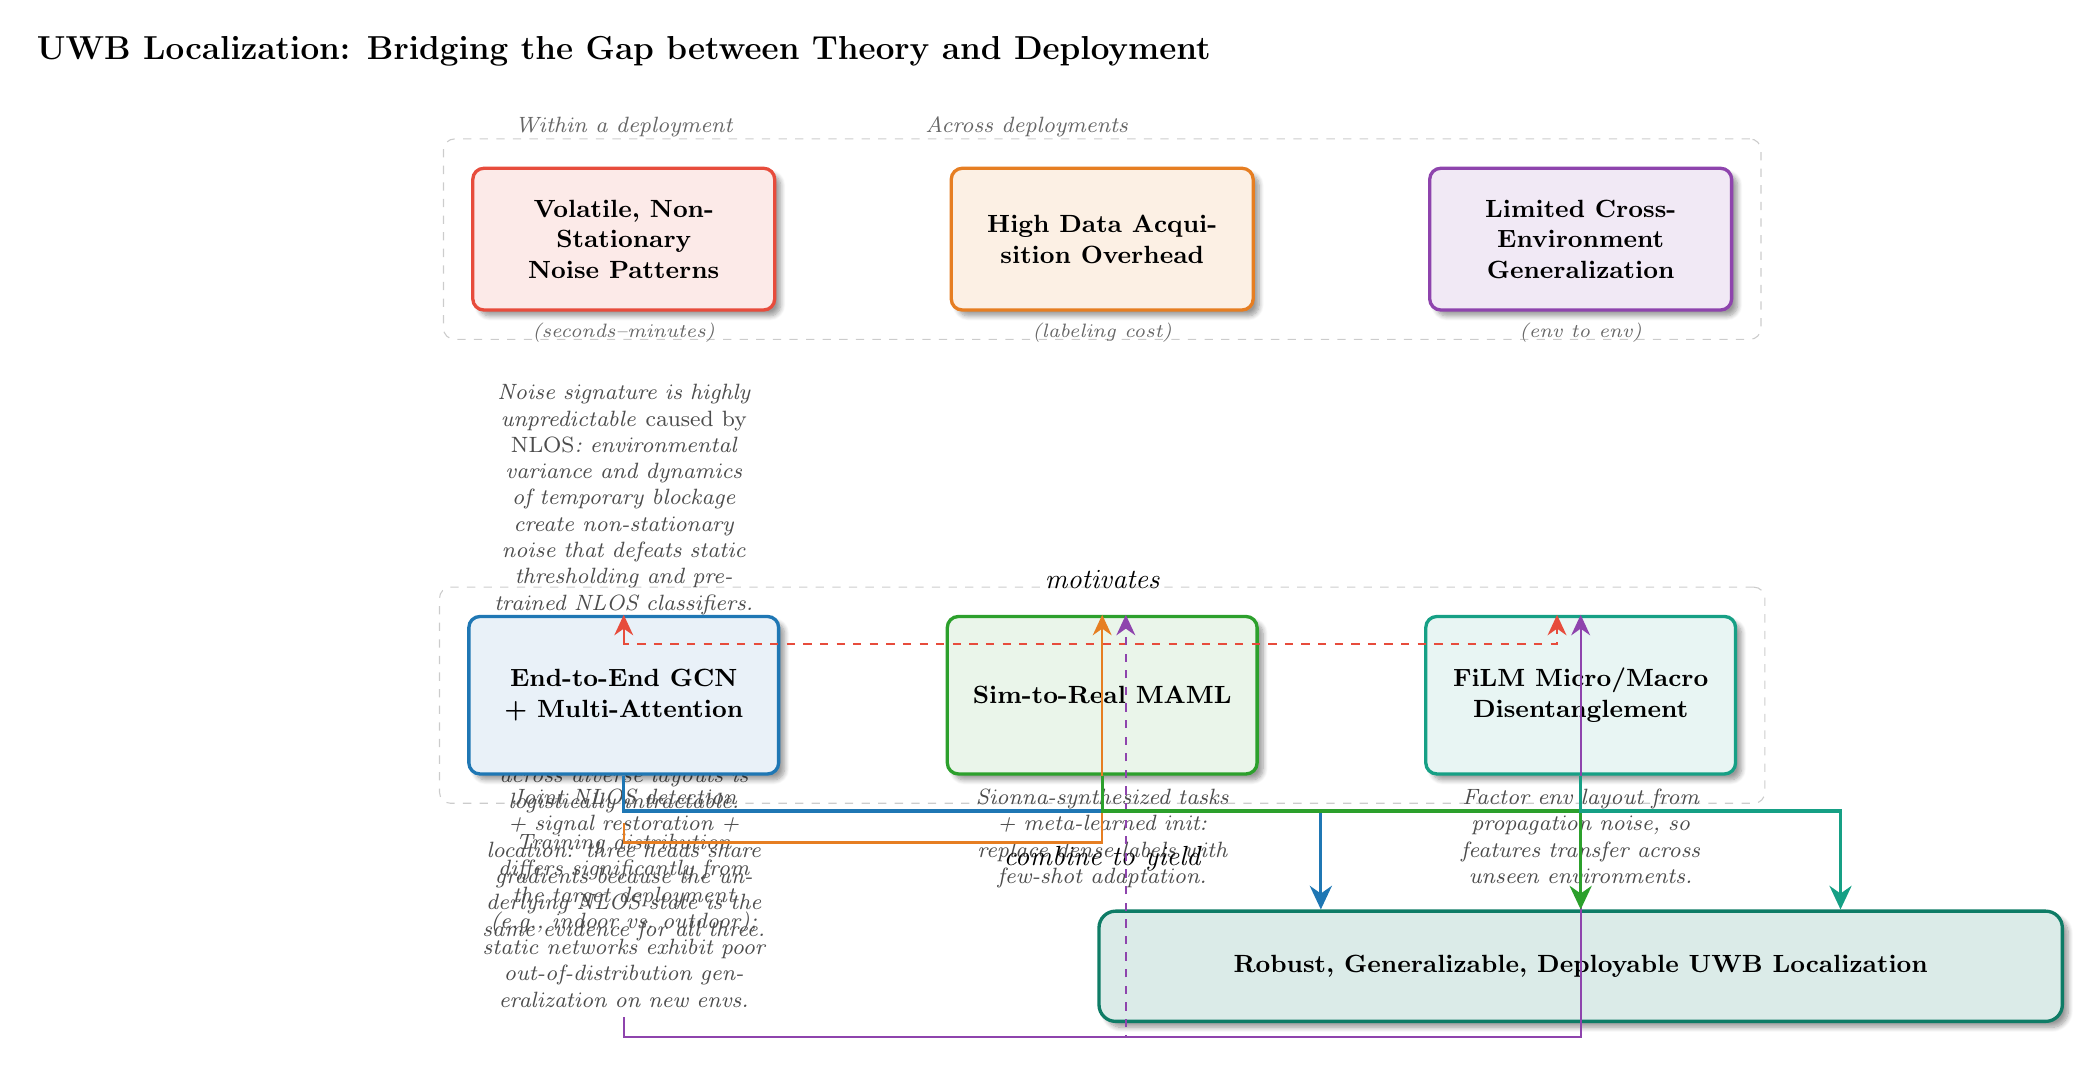
\begin{tikzpicture}[node distance=0.6cm and 0.7cm]

  % --- Title strip ---
  \node[font=\bfseries\large] (title) at (0, 0) {UWB Localization: Bridging the Gap between Theory and Deployment};

  % --- Time-scale axis (above challenges) ---
  \node[font=\footnotesize\itshape, text=black!60, below=0.4cm of title] (ax1) {Within a deployment};
  \node[font=\footnotesize\itshape, text=black!60, right=2.2cm of ax1] (ax2) {Across deployments};

  % --- Three Challenges ---
  \node[challenge=challengeA, below=0.25cm of ax1] (c1) {Volatile, Non-Stationary Noise Patterns};
  \node[timescale, below=0.02cm of c1] {(seconds--minutes)};

  \node[challenge=challengeB, right=2.2cm of c1] (c2) {High Data Acquisition Overhead};
  \node[timescale, below=0.02cm of c2] {(labeling cost)};

  \node[challenge=challengeC, right=2.2cm of c2] (c3) {Limited Cross-Environment Generalization};
  \node[timescale, below=0.02cm of c3] {(env to env)};

  % --- Sub-captions (your phrasings, lightly trimmed) ---
  \node[label, text width=3.6cm, below=0.25cm of c1, yshift=-0.55cm] (lc1) {Noise signature is highly unpredictable \emph{caused by NLOS}: environmental variance and dynamics of temporary blockage create non-stationary noise that defeats static thresholding and pre-trained NLOS classifiers.};
  \node[label, text width=3.6cm, below=0.02cm of lc1] (lc2) {Supervised models need vast, precisely labeled data to cover the full noise spectrum; obtaining dense ground-truth across diverse layouts is logistically intractable.};
  \node[label, text width=3.6cm, below=0.02cm of lc2] (lc3) {Training distribution differs significantly from the target deployment (e.g., indoor vs.\ outdoor); static networks exhibit poor out-of-distribution generalization on new envs.};

  % --- "Motivates" arrow group ---
  \node[font=\itshape] at ($(c1.south)!0.5!(c3.south) + (0,-3.4)$) {motivates};

  % --- Three Solution Pillars ---
  \node[solution=solution1, below=3.85cm of c1] (s1) {End-to-End GCN + Multi-Attention};
  \node[label, text width=3.7cm, below=0.05cm of s1] {Joint NLOS detection + signal restoration + location: three heads share gradients because the underlying NLOS state is the same evidence for all three.};

  \node[solution=solution2, below=3.85cm of c2] (s2) {Sim-to-Real MAML};
  \node[label, text width=3.7cm, below=0.05cm of s2] {Sionna-synthesized tasks + meta-learned init: replace dense labels with few-shot adaptation.};

  \node[solution=solution3, below=3.85cm of c3] (s3) {FiLM Micro/Macro Disentanglement};
  \node[label, text width=3.7cm, below=0.05cm of s3] {Factor env layout from propagation noise, so features transfer across unseen environments.};

  % --- "Combine to yield" caption ---
  \node[font=\itshape] at ($(s1.south)!0.5!(s3.south) + (0,-1.05)$) {combine to yield};

  % --- Final Outcome ---
  \node[outcome, below=1.6cm of s3, yshift=-0.1cm] (out) {Robust, Generalizable, Deployable UWB Localization};

  % --- Arrows: challenges -> solutions (primary + supporting) ---
  % C1 (volatile, within-deployment) -> S1 (end-to-end GCN, primary)
  \draw[arr, challengeA] (lc1.south) -- ++(0,-0.25) -| (s1.north);
  % C1 also -> S3 (FiLM): noise statistics also vary across envs
  \draw[arr, challengeA, dashed] (lc1.south) -- ++(0,-0.25) -| ([xshift=-0.3cm]s3.north);
  % C2 (data) -> S2 (MAML, primary)
  \draw[arr, challengeB] (lc2.south) -- ++(0,-0.25) -| (s2.north);
  % C3 (cross-env) -> S3 (FiLM, primary)
  \draw[arr, challengeC] (lc3.south) -- ++(0,-0.25) -| (s3.north);
  % C3 also -> S2 (MAML): cross-env init also needs meta-learning
  \draw[arr, challengeC, dashed] (lc3.south) -- ++(0,-0.25) -| ([xshift=0.3cm]s2.north);

  % --- Arrows: solutions -> outcome ---
  \draw[arrbold, solution1] (s1.south) -- ++(0,-0.45) -| ([xshift=-3.3cm]out.north);
  \draw[arrbold, solution2] (s2.south) -- ++(0,-0.45) -| (out.north);
  \draw[arrbold, solution3] (s3.south) -- ++(0,-0.45) -| ([xshift=3.3cm]out.north);

  % --- Brace-style grouping labels ---
  \begin{scope}[on background layer]
    \node[draw=gray!40, dashed, rounded corners=4pt, fit=(c1)(c2)(c3),
          inner sep=10pt, label={[font=\bfseries, gray!70]above:Technical Challenges}] {};
    \node[draw=gray!40, dashed, rounded corners=4pt, fit=(s1)(s2)(s3),
          inner sep=10pt, label={[font=\bfseries, gray!70]above:Our Framework}] {};
  \end{scope}

\end{tikzpicture}
\end{center}

\bigskip

\noindent\textbf{Three core challenges} motivate our design. We distinguish them by where in the deployment lifecycle the failure occurs:

\begin{description}[leftmargin=1.8cm, style=nextline]
  \item[\textbf{Volatile, Non-Stationary Noise Patterns.}] Real-world UWB deployments suffer from highly unpredictable noise signature caused by NLOS: variance of environment and dynamics of temporay blockage create non-stationary noise characteristics that cause static thresholding and pre-trained Non-Line-of-Sight (NLOS) classifiers to fail.

  \item[\textbf{High Data Acquisition Overhead.}] Supervised deep learning models require vast quantities of precisely labeled data to capture the full spectrum of environmental noise patterns. However, obtaining dense, accurate ground-truth NLOS features and coordinates across diverse physical layouts and dynamic configurations is logistically complex and labor-intensive, creating a severe bottleneck for practical model training.

  \item[\textbf{Limited Cross-Environment Generalization.}] Due to unpredictable spatial variations, a model's training distribution can differ significantly from its target deployment setting (e.g., indoor vs outdoor). Static localization networks exhibit poor out-of-distribution generalization, experiencing severe performance degradation when introduced to new, unmapped environments with distinct multipath characteristics.
\end{description}

\noindent Our framework systematically overcomes these challenges by introducing three core technical components, each addressing a different axis of distribution shift:

\begin{enumerate}
  \item \textbf{End-to-end Localization System with Dual-Channel GCN and Multi-Attention Mechanism (addresses volatile noise):} Our unified end-to-end architecture leverages data redundancy across cooperative sensors by jointly performing NLOS detection, signal restoration, and coordinate regression in a single network instead of utilizing isolated stages. Because these three tasks are tightly coupled in physical propagation---the same NLOS condition that biases a range measurement is also the one that should be downweighted by the restoration head and flagged by the detector---an end-to-end formulation lets gradients flow between them so each head benefits from the others' evidence. Formulated as a graph network, the architecture maps three distinct dimensions of dependencies: dynamic weight matrices preserve environment-independent cross-sensor interactions and encode the hidden physical constraints between heterogeneous channels (radial distance vs.\ directional angle), while a multi-head self-attention module extracts global sensor relationships. This joint reasoning enables the network to implicitly filter complex noise and reconstruct clean measurements end-to-end.

  \item \textbf{Simulation-to-Reality Meta-Learning via MAML (addresses data overhead):} To circumvent real-world data collection limits and guarantee spatial generalization, we utilize the Sionna ray-tracing emulation platform to generate high-fidelity, labeled UWB datasets across diverse virtual topologies. We then employ Model-Agnostic Meta-Learning (MAML) to pre-train the network on these varied environmental tasks. This optimization enables the base model to learn highly transferable feature representations, allowing it to adapt to novel, real-world target scenarios using only a few-shot support set of local reference samples.

  \item \textbf{FiLM-based Micro/Macro Disentanglement (addresses cross-environment generalization):} Beyond the meta-learned initialization, we introduce a FiLM-conditioned micro-condition representation $c$ that captures the local propagation state (e.g., NLOS severity per anchor) while a gradient-reversal adversary forces $c$ to be uninformative about the macro environment. At test time, the model composes the macro environment (from the meta-learned features) and the micro propagation condition (from $c$) on the fly, so features learned in one environment can re-combine with the new environment's local noise conditions.
\end{enumerate}

\noindent By integrating these three techniques, our model mitigates moment-to-moment noise through in-network restoration, reduces the labeling burden through synthetic meta-pretraining, and achieves environment-agnostic feature transfer through disentangled composition.

\end{document}
